\section{Vantaggi di Redpanda}
\subsection{Performance}
Redpanda è scritto in C++ e utilizza il \textit{framework} Seastar, offrendo un'architettura \textit{thread-per-core} ad alte prestazioni.
Ciò permette di ottenere un'elevata \textit{throughput} e latenze costantemente basse, evitando cambi di contesto e blocchi.
Inoltre, è progettato per sfruttare l'\textit{hardware} moderno, tra cui unità NVMe, processori \textit{multi-core} e interfacce di rete ad alta velocità.

\subsection{Costi}
Anche per carichi di lavoro ridotti, l'utilizzo di Kafka può essere \href{https://redpanda.com/blog/is-redpanda-better-than-kafka-tco-comparison}{fino a 3 volte più costoso} rispetto a Redpanda. Per carichi di lavoro più complessi, questa differenza può aumentare fino a 5 volte o più.\\

\subsection{Semplicità di configurazione}
Redpanda è un contenuto in un singolo binario. Lo \textit{schema registry}, il \textit{proxy} HTTP e il \textit{message broker} sono tutti integrati. Ciò significa che non ci sono dipendenze da JVM, ZooKeeper o KRaft.

\subsection{BYOC (\textit{Bring Your Own Cluster})}
Redpanda offre una terza opzione oltre alla gestione autonoma di un \textit{cluster} di \textit{streaming}
dati e all'utilizzo di un servizio \textit{cloud} completamente gestito: \textit{Bring Your Own Cluster} (BYOC).
Questa alternativa consente agli utenti finali di implementare una soluzione parzialmente gestita dal fornitore nella propria infrastruttura (come il proprio \textit{data center}
o il proprio \textit{VPC cloud}).\\

\subsection{Compatibilità con API di Kafka}
Redpanda è progettato per essere compatibile con le API di Kafka, consentendo di utilizzare i \textit{client} Kafka esistenti senza modifiche.

\subsection{\textit{Self-healing}}
Redpanda è self-healing e redistribuisce continuamente i dati e la \textit{leadership} tra i nodi per mantenere il \textit{cluster} in uno stato ottimale mentre il \textit{cluster} evolve o quando i nodi falliscono.

\subsection{Architettura e Sicurezza}
La versione più recente di Kafka ha introdotto KRaft come sostituto di Apache ZooKeeper. KRaft, come suggerisce il nome, sfrutta il protocollo Raft per gestire i metadati del \textit{cluster}.
KRaft è stato marcato come pronto per la produzione in Apache Kafka 3.4.0. Tuttavia, alcune limitazioni rimangono, tra cui:

\begin{itemize}
	\item Nessuna possibilità di aggiornare i \textit{cluster} esistenti da ZooKeeper a KRaft
	\item Nessun supporto per l'autenticazione SASL/SCRAM
	\item Modifiche al \textit{tooling} da riga di comando che non funzionano con TLS
\end{itemize}
Con KRaft, solo i metadati e lo stato del \textit{cluster} sono memorizzati nel \textit{quorum} di KRaft, mentre i \textit{topic} e le partizioni utilizzano ancora il meccanismo ISR.\\
Per contrasto invece, Redpanda utilizza Raft per la configurazione del \textit{cluster}, lo stato e il mantenimento del consenso attorno alle repliche delle partizioni. Questo utilizzo di Raft per la replicazione consente a Redpanda di offrire garanzie di sicurezza dei dati superiori e di evitare scenari documentati in cui Kafka può perdere lo stato e richiedere un'elezione del \textit{leader} non
sicura.
\\
\href{https://redpanda.com/blog/kafka-kraft-vs-redpanda-performance-2023}{Fonte}


\begin{center}
	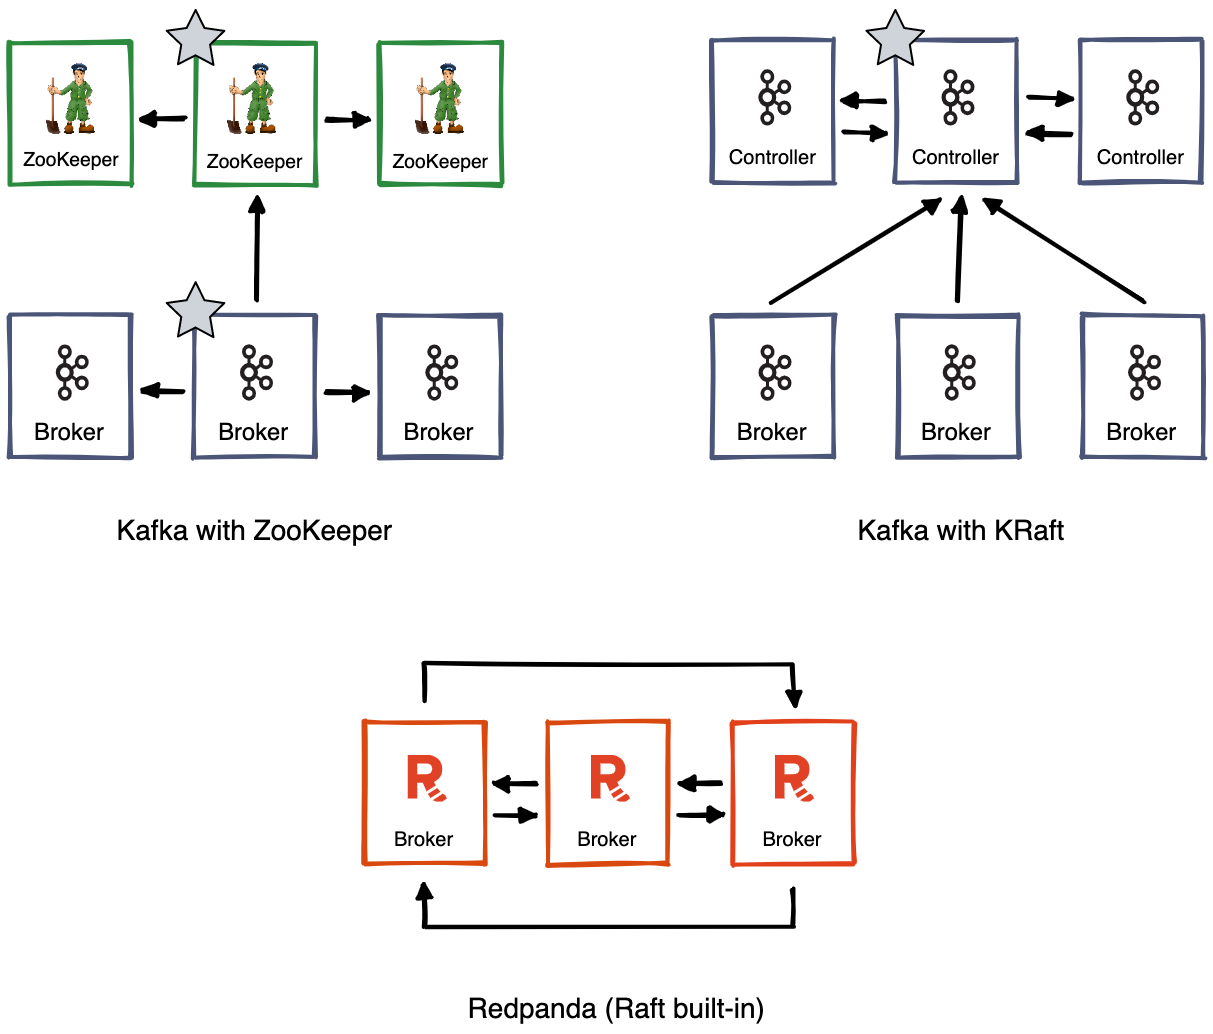
\includegraphics[width=0.65\textwidth]{imgs/kafka_zookeeper.png}
\end{center}


